% 41039 Programming 1 -- Revision of Week 4
% Shown at the start of the next lecture, before any new material.
% Scope: the Week 4 page (weeks/week-4.html), sections 01-08 -- methods, return, overloading,
% varargs, Python functions and parameters, the call stack and the heap, pass-by-value in
% Java and call-by-object-reference in Python, records. There is no Lecture 4 deck.
% Two parts: six individual questions, then four team rounds (draw the memory, spot the
% errors, predict the output, write the code).
% Style and macros are identical to revision-week-3.tex, with stack/heap TikZ styles.
% Compile: xelatex revision-week-4.tex   (run twice; bk-logo.png sits next to this file)

\documentclass[aspectratio=169]{beamer}
\makeatletter

\usepackage{lmodern}
\usepackage{booktabs}
\usepackage{array}
\usepackage{graphicx}
\usepackage{xcolor}
\usepackage{listings}
\usepackage{pifont}
\usepackage{enumitem}
\usepackage[most]{tcolorbox}
\usepackage{tikz}
\usetikzlibrary{shapes.geometric, arrows.meta, positioning}

% Beamer's default enumerate label expands to itself once enumitem takes the optional
% argument, and TeX runs out of input stack. An explicit label breaks the loop.
\setlist[enumerate]{label=\arabic*.}
\setlist[itemize]{label=\usebeamertemplate{itemize item}}

\definecolor{bkblue}{RGB}{0,70,140}
\definecolor{bktitlebg}{RGB}{64,116,169}
\definecolor{codebg}{RGB}{244,246,249}
\definecolor{codecmt}{RGB}{110,120,130}
\definecolor{codegray}{RGB}{110,120,135}
\definecolor{codestr}{RGB}{150,60,20}
\definecolor{badred}{RGB}{185,40,40}
\definecolor{goodgreen}{RGB}{20,125,70}
\definecolor{srcgrey}{RGB}{105,115,128}

\usetheme{default}
\useinnertheme{rounded}
\setbeamertemplate{navigation symbols}{}

\setbeamercolor{titlelike}{bg=bktitlebg,fg=white}
\setbeamercolor{frametitle}{fg=bkblue,bg=}
\setbeamercolor{author}{fg=bkblue}
\setbeamercolor{institute}{fg=bkblue}
\setbeamercolor{section in toc}{fg=bkblue}
\setbeamerfont{frametitle}{size=\Large,series=\mdseries}
\setbeamerfont{title}{size=\Large,series=\bfseries}
\setbeamerfont{subtitle}{size=\normalsize,series=\bfseries}

\setbeamertemplate{frametitle}{%
  \vspace*{0.35em}%
  \begin{minipage}[b]{0.84\textwidth}%
    \usebeamerfont{frametitle}\usebeamercolor[fg]{frametitle}\insertframetitle%
  \end{minipage}\hfill%
  \begin{minipage}[b]{0.10\textwidth}%
    \raggedleft
\includegraphics[height=0.75cm]{bk-logo.png}%
  \end{minipage}\\[0.1em]%
  {\color{bkblue}\rule{\textwidth}{0.7pt}}%
}

\setbeamercolor{footbar}{bg=bkblue,fg=white}
\setbeamertemplate{footline}{%
  \begin{beamercolorbox}[wd=\paperwidth,ht=2.1ex,dp=1.1ex,leftskip=.3cm,rightskip=.3cm]{footbar}%
    \tiny\insertshorttitle\hfill\insertframenumber{}/\inserttotalframenumber%
  \end{beamercolorbox}%
}

\newcommand{\keyline}[1]{\vfill\begin{center}\textcolor{bkblue}{\textbf{#1}}\end{center}\vspace*{0.2em}}
\newcommand{\hd}[1]{\textbf{#1}}
\newcommand{\code}[1]{\texttt{#1}}
\newcommand{\srcline}[1]{{\color{srcgrey}\scriptsize #1\par}}
\newcommand{\srclink}[2]{\href{#1}{\texttt{#2}}}
\newcommand{\badlabel}[1]{\textcolor{badred}{\ding{55}~\textbf{#1}}}
\newcommand{\goodlabel}[1]{\textcolor{goodgreen}{\ding{51}~\textbf{#1}}}
\newcommand{\neutrallabel}[1]{\textcolor{bkblue}{\textbf{#1}}}
\newcommand{\timing}[2]{\hfill{\small\textcolor{bkblue}{\textbf{#1 \textbullet{} #2}}}}
% a blank to be filled in, numbered so the word bank can be checked against it
\newcommand{\blank}[1]{\underline{\hspace{1.1em}\textbf{(#1)}\hspace{1.1em}}}
\newcommand{\yes}{\textcolor{goodgreen}{\ding{51}}}
\newcommand{\no}{\textcolor{badred}{\ding{55}}}

% --- Stack and heap pictures (Draw it) --------------------------------------
\tikzset{
  sframe/.style={draw=bkblue, thick, fill=codebg, rounded corners=2pt, inner sep=4pt,
    font=\scriptsize\ttfamily, align=left, anchor=north west},
  ftitle/.style={font=\scriptsize\sffamily\bfseries, text=bkblue, anchor=south west},
  cell/.style={draw=bkblue, fill=white, font=\scriptsize\ttfamily, minimum width=0.62cm,
    minimum height=0.5cm, inner sep=1pt},
  atitle/.style={font=\scriptsize\ttfamily, text=bkblue, anchor=south west, inner sep=1pt},
  ref/.style={-{Stealth[length=5pt]}, thick, draw=bkblue!85!black},
  hd/.style={font=\small\sffamily\bfseries, text=bkblue},
}

\hypersetup{colorlinks=true, urlcolor=bkblue, linkcolor=bkblue}

% --- Question box: what the room is being asked --------------------------
\newtcolorbox{discussionbox}[1]{
  title=\textbf{#1}, coltitle=bkblue, colback=white, colframe=bkblue,
  colbacktitle=bkblue!10, boxrule=1pt, arc=3pt,
  left=6pt, right=6pt, top=4pt, bottom=4pt
}
% --- Answer box: revealed after they have committed to an answer ---------
\newtcolorbox{contextbox}[1]{
  title=\textbf{#1}, coltitle=white, colback=bkblue!5, colframe=bkblue,
  colbacktitle=bkblue!80, boxrule=0.6pt, arc=3pt,
  left=6pt, right=6pt, top=4pt, bottom=4pt
}

\lstdefinestyle{code}{
  basicstyle=\ttfamily\scriptsize,
  keywordstyle=\color{bkblue}\bfseries,
  commentstyle=\color{codecmt}\itshape,
  stringstyle=\color{codestr},
  backgroundcolor=\color{codebg},
  frame=leftline, framerule=1.2pt, rulecolor=\color{bkblue},
  xleftmargin=1.1em, framexleftmargin=1.1em,
  framexrightmargin=0.4em, framextopmargin=3pt, framexbottommargin=3pt,
  showstringspaces=false, columns=fullflexible, keepspaces=true,
  breaklines=true, aboveskip=0.6em, belowskip=0.6em,
}
\lstdefinestyle{bad}{style=code, rulecolor=\color{badred}, backgroundcolor=\color{badred!4}}
\lstdefinestyle{good}{style=code, rulecolor=\color{goodgreen}, backgroundcolor=\color{goodgreen!5}}
\lstset{style=code}
% listings' Python predates 3.10; teach it the soft keywords and constants this deck uses
\lstdefinelanguage{Py}[]{Python}{morekeywords={match,case,elif,True,False}}

\setbeamertemplate{title page}{%
  \vspace*{0.5em}
  \begin{centering}
    \begin{beamercolorbox}[sep=8pt,center,rounded=true,shadow=false]{title}
      \usebeamerfont{title}\inserttitle\par
      \ifx\insertsubtitle\@empty\else
        \vskip0.4em{\usebeamerfont{subtitle}\insertsubtitle\par}
      \fi
    \end{beamercolorbox}
    \vskip1.0em
    
\includegraphics[height=1.7cm]{bk-logo.png}
    \vskip1.0em
    {\usebeamercolor[fg]{author}\usebeamerfont{author}\insertauthor\par}
    \vskip0.5em
    {\usebeamercolor[fg]{institute}\usebeamerfont{institute}\insertinstitute\par}
    \vskip0.6em
    {\usebeamerfont{date}\insertdate\par}
  \end{centering}
}



\title[41039 Programming 1 --- Revision of Week 4]{41039 Programming 1}
\subtitle{Revision of Week 4: methods, functions, the stack and the heap, and records}
\author{Dr. Xuan-Bach Le\\ \small\texttt{le.xuan.bach@hcmut.edu.vn}}
\institute{\small Faculty of Computer Science and Engineering, HCMUT}
\date{September Session 2026}

\AtBeginSection[]{%
  \begin{frame}{Outline}
    \tableofcontents[currentsection]
  \end{frame}%
}

\begin{document}

\begin{frame}[plain]
  \titlepage
\end{frame}

% ======================================================================
\begin{frame}{How the next fifty minutes work}
  \hd{Same deal as before.} Not a test. Nothing is recorded against you. Answering earns
  extra credit, and being wrong out loud earns it too.
  \vspace{0.5em}
  \begin{columns}[T,onlytextwidth]
    \column{0.47\textwidth}
    \neutrallabel{Part 1 --- on your own}
    \begin{itemize}[itemsep=0.2em]
      \small
      \item Six short questions, about a minute each
      \item Commit to an answer \textbf{before} the reveal: on paper, or out loud
    \end{itemize}
    \column{0.49\textwidth}
    \neutrallabel{Part 2 --- in teams of 3 or 4}
    \begin{itemize}[itemsep=0.2em]
      \small
      \item Four rounds: \textbf{draw the memory}, \textbf{spot the errors},
        \textbf{predict the output}, \textbf{write the code}
      \item One sheet of paper, one spokesperson. Every team that reports back earns credit
      \item The last one goes to the keyboard: one Java team, one Python team
    \end{itemize}
  \end{columns}
  \vspace{0.4em}
  \hd{These are hard on purpose.} Which variable is this? Which frame is it in? Does the
  caller ever see the change? If you are drawing boxes and arrows, you are doing it right.
  \keyline{For every method call: what is copied, and what is shared?}
\end{frame}

% ======================================================================
\section{On your own}
% ======================================================================

\begin{frame}[fragile]{Which of these compile? \timing{Alone}{90 seconds}}
  \begin{columns}[T,onlytextwidth]
    \column{0.54\textwidth}
\begin{lstlisting}[language=Java]
static int sign(int n) {            // (a)
    if (n > 0) return 1;
    else if (n < 0) return -1;
}
static boolean even(int n) {        // (b)
    return n % 2;
}
static void hello() { return; }     // (c)
static int twice(int n) {           // (d)
    return n * 2;
    System.out.println("done");
}
\end{lstlisting}
    \column{0.42\textwidth}
    \pause
    \begin{contextbox}{Answers}
      \footnotesize\raggedright
      \textbf{(a)} \no{} \code{missing return statement}. When \code{n} is 0, no
      \code{return} is reached. Add \code{else return 0;}\\[0.3em]
      \textbf{(b)} \no{} \code{n \% 2} is an \code{int}, not a \code{boolean}:
      \code{return n \% 2 == 0;}\\[0.3em]
      \textbf{(c)} \yes{} a \code{void} method may \code{return} early, with no value.
      \code{return 0;} would not compile: \code{unexpected return value}\\[0.3em]
      \textbf{(d)} \no{} \code{unreachable statement}. \code{return} ends the method;
      nothing after it can run
    \end{contextbox}
  \end{columns}
  \keyline{The compiler checks every path. It never checks that the answer is right.}
\end{frame}

\begin{frame}[fragile]{Which one runs? \timing{Alone}{60 seconds}}
  \begin{columns}[T,onlytextwidth]
    \column{0.52\textwidth}
\begin{lstlisting}[language=Java]
static void show(int x)
    { System.out.println("int " + x); }
static void show(double x)
    { System.out.println("double " + x); }
static void show(int x, int y)
    { System.out.println("two " + (x + y)); }
static void show(int... xs)
    { System.out.println("varargs " + xs.length); }
\end{lstlisting}
    \begin{discussionbox}{What prints?}
      \small
      \code{show(5);} \code{show(5.0);} \code{show(2, 3);} \code{show(1, 2, 3);}
      \code{show();}\\[0.2em]
      \textbf{And:} could you add \code{static int show(int x)}?
    \end{discussionbox}
    \column{0.44\textwidth}
    \pause
    \begin{contextbox}{Answers}
      \footnotesize\raggedright
      \code{int 5} --- the exact match wins\\[0.15em]
      \code{double 5.0}\\[0.15em]
      \code{two 5} --- two \code{int}s: the two-parameter version\\[0.15em]
      \code{varargs 3} --- only varargs takes three\\[0.15em]
      \code{varargs 0} --- varargs accepts \textbf{zero} values\\[0.35em]
      \textbf{No:} \code{method show(int) is already defined}. Overloads must differ in
      their \textbf{parameter lists}; the return type does not count
    \end{contextbox}
  \end{columns}
\end{frame}

\begin{frame}[fragile]{Three variables called \texttt{n} \timing{Alone}{90 seconds}}
  \hd{1.} What prints? \quad \hd{2.} Just before \code{g} returns: how many frames, and
  what is each \code{n}?
  \vspace{-0.3em}
  \begin{columns}[T,onlytextwidth]
    \column{0.50\textwidth}
\begin{lstlisting}[language=Java]
static int f(int n) {
    n = n * 2;
    return g(n) + n;
}
static int g(int n) {
    n = n + 1;
    return n;
}
public static void main(String[] args) {
    int n = 3;
    int r = f(n);
    System.out.println(n + " " + r);
}
\end{lstlisting}
    \column{0.46\textwidth}
    \pause
    \begin{contextbox}{Answers}
      \footnotesize\raggedright
      \textbf{1.} \code{3 13}. \code{f} doubles \emph{its} \code{n} to 6; \code{g} makes
      \emph{its} \code{n} 7 and returns 7; \code{f} returns 7 + 6. \code{main}'s \code{n}
      was copied, never changed\\[0.2em]
      \textbf{2.} Three frames, three separate \code{n}s:
    \end{contextbox}
    \vspace{0.1em}
    \begin{center}
    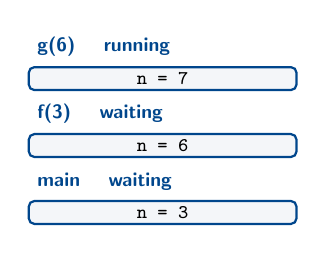
\begin{tikzpicture}
      \node[sframe, minimum width=3.4cm, inner sep=2pt] (g) at (0,0) {n = 7};
      \node[ftitle] at (g.north west) {g(6) \quad running};
      \node[sframe, minimum width=3.4cm, inner sep=2pt] (f) at (0,-0.85) {n = 6};
      \node[ftitle] at (f.north west) {f(3) \quad waiting};
      \node[sframe, minimum width=3.4cm, inner sep=2pt] (m) at (0,-1.7) {n = 3};
      \node[ftitle] at (m.north west) {main \quad waiting};
    \end{tikzpicture}
    \end{center}
  \end{columns}
\end{frame}

\begin{frame}[fragile]{Mutate, or reassign? \timing{Alone}{90 seconds}}
  \begin{columns}[T,onlytextwidth]
    \column{0.50\textwidth}
\begin{lstlisting}[language=Java]
static void a(int[] v) { v[0] = 9; }
static void b(int[] v)
    { v = new int[] {7, 7}; }
static void c(int[] v) {
    v = new int[] {5, 5};
    v[1] = 1;
}
static int[] d(int[] v) {
    v = new int[] {4, 4};
    return v;
}
\end{lstlisting}
    \column{0.46\textwidth}
\begin{lstlisting}[language=Java]
int[] x = {1, 2};
a(x);        // x is now?
b(x);        // x is now?
c(x);        // x is now?
x = d(x);    // x is now?
int[] y = x;  y[1] = 0;   // x?
\end{lstlisting}
    \pause
    \begin{contextbox}{Answers}
      \scriptsize\raggedright
      \code{a}: \code{\{9, 2\}} --- \code{v} is a copy of the \emph{reference}\\
      \code{b}: \code{\{9, 2\}} --- reassigning \code{v} re-points only the copy\\
      \code{c}: \code{\{9, 2\}} --- \code{v[1] = 1} changed the \emph{new} array\\
      \code{d}: \code{\{4, 4\}} --- \code{main} assigned the returned reference\\
      \code{y[1] = 0}: \code{\{4, 0\}} --- two names, one array
    \end{contextbox}
  \end{columns}
\end{frame}

\begin{frame}[fragile]{Python: what does the caller see? \timing{Alone}{90 seconds}}
  \begin{columns}[T,onlytextwidth]
    \column{0.48\textwidth}
\begin{lstlisting}[language=Py]
# (a)
def f(items, n):
    items += [n]
    n += 1
    items = items + [n]

nums = [1]
k = 5
r = f(nums, k)
print(nums, k, r)

# (b)
print(print("x"))
\end{lstlisting}
    \column{0.48\textwidth}
    \pause
    \begin{contextbox}{Answers}
      \footnotesize\raggedright
      \textbf{(a)} \code{[1, 5] 5 None}\\[0.15em]
      \code{items += [n]} \textbf{mutates} the list, so \code{nums} sees it.\\
      \code{n += 1} makes a new number, for the local \code{n} only.\\
      \code{items = items + [n]} builds a \textbf{new} list and rebinds the local name.\\
      No \code{return}, so \code{r} is \code{None}\\[0.35em]
      \textbf{(b)} \code{x}, then \code{None}. The inner \code{print} shows \code{x} and
      returns \code{None}; the outer one prints that
    \end{contextbox}
  \end{columns}
  \keyline{+= on a list mutates it. x = x + [...] builds a new one.}
\end{frame}

\begin{frame}[fragile]{Records: compile, and print what? \timing{Alone}{60 seconds}}
  \begin{columns}[T,onlytextwidth]
    \column{0.52\textwidth}
\begin{lstlisting}[language=Java]
record Point(int x, int y) {}

Point p = new Point(1, 2);
System.out.println(p);               // (a)
System.out.println(p.x() + p.y());   // (b)
p.x = 5;                             // (c)
Point q = new Point(1);              // (d)
p = new Point(3, 4);                 // (e)
System.out.println(p);
\end{lstlisting}
    {\small Records need Java 16 or later: run these on Ed, not in the site's console.}
    \column{0.44\textwidth}
    \pause
    \begin{contextbox}{Answers}
      \footnotesize\raggedright
      \textbf{(a)} \code{Point[x=1, y=2]} --- printing comes free\\[0.25em]
      \textbf{(b)} \code{3} --- components are read with \emph{methods}: \code{p.x()}\\[0.25em]
      \textbf{(c)} \no{} \code{cannot assign a value to final variable x}. A record's
      components never change\\[0.25em]
      \textbf{(d)} \no{} the constructor takes \textbf{both} components, in order\\[0.25em]
      \textbf{(e)} \yes{} prints \code{Point[x=3, y=4]}. The \emph{Point} cannot change,
      but the \emph{variable} \code{p} can refer to a different one
    \end{contextbox}
  \end{columns}
  \keyline{A final component is not a final variable. Know which one you have.}
\end{frame}

% ======================================================================
\section{Team round 1: draw the memory}
% ======================================================================

\begin{frame}{Form teams}
  \begin{columns}[T,onlytextwidth]
    \column{0.48\textwidth}
    \neutrallabel{Now}
    \begin{itemize}[itemsep=0.3em]
      \item Teams of \textbf{3 or 4}, with the people next to you
      \item One sheet of paper. Write the team's names on it
      \item Pick a \textbf{spokesperson} --- a different one for each challenge, if you can
    \end{itemize}
    \column{0.48\textwidth}
    \neutrallabel{For each challenge}
    \begin{itemize}[itemsep=0.3em]
      \item The timer is on the slide
      \item When it runs out, one team is called on to answer. Others may disagree ---
        \textbf{disagreeing with a reason also earns credit}
      \item ``I think it's X \emph{because}\ldots'' beats ``X''
    \end{itemize}
  \end{columns}
  \vspace{0.6em}
  \begin{contextbox}{How to draw memory}
    \small Stack on the left: one box per method call, newest on top, holding that call's
    parameters and local variables. Heap on the right: every array or object made with
    \code{new}. An arrow for every reference. Numbers and \code{boolean}s sit in the box
    itself.
  \end{contextbox}
\end{frame}

\begin{frame}[fragile]{Draw it: the stack and the heap \timing{Teams}{5 min}}
  \begin{columns}[T,onlytextwidth]
    \column{0.52\textwidth}
\begin{lstlisting}[language=Java]
static int[] tally(int[] marks, int pass) {
    int[] counts = new int[2];
    for (int m : marks) {
        if (m >= pass) counts[1]++;
        else counts[0]++;
    }
    // (*) draw the stack and the heap HERE
    return counts;
}
public static void main(String[] args) {
    int[] marks = {72, 45, 91};
    int pass = 50;
    int[] result = tally(marks, pass);
    System.out.println(result[0] + " fail");
    System.out.println(result[1] + " pass");
}
\end{lstlisting}
    \column{0.44\textwidth}
    \begin{discussionbox}{Draw it, then answer}
      \small
      \textbf{1.} Draw the stack and the heap at \code{(*)}. Every variable, every array,
      every arrow.\\[0.3em]
      \textbf{2.} How many variables are called \code{marks}? How many arrays hold
      72, 45, 91?\\[0.3em]
      \textbf{3.} Where is \code{m} at \code{(*)}?\\[0.3em]
      \textbf{4.} Redraw it just after \code{tally} returns. What has gone, and what
      survived? What prints?
    \end{discussionbox}
  \end{columns}
\end{frame}

\begin{frame}{Draw it: one answer}
  \begin{columns}[T,onlytextwidth]
    \column{0.62\textwidth}
    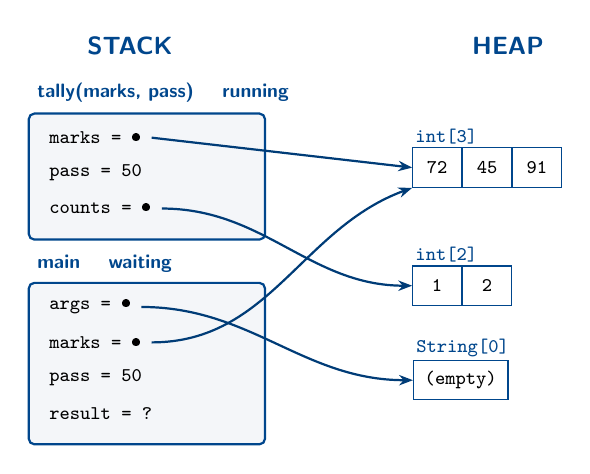
\begin{tikzpicture}
      \node[hd] at (1.3,0.55) {STACK};
      \node[hd] at (6.1,0.55) {HEAP};
      % frames
      \node[sframe, minimum width=3.0cm, minimum height=1.6cm] (t) at (0,-0.3) {};
      \node[ftitle] at (t.north west) {tally(marks, pass) \quad running};
      \node[font=\scriptsize\ttfamily, anchor=west] (tm) at (0.15,-0.62) {marks = \textbullet};
      \node[font=\scriptsize\ttfamily, anchor=west] (tp) at (0.15,-1.07) {pass = 50};
      \node[font=\scriptsize\ttfamily, anchor=west] (tc) at (0.15,-1.52) {counts = \textbullet};
      \node[sframe, minimum width=3.0cm, minimum height=2.05cm] (mf) at (0,-2.45) {};
      \node[ftitle] at (mf.north west) {main \quad waiting};
      \node[font=\scriptsize\ttfamily, anchor=west] (ma) at (0.15,-2.77) {args = \textbullet};
      \node[font=\scriptsize\ttfamily, anchor=west] (mm) at (0.15,-3.22) {marks = \textbullet};
      \node[font=\scriptsize\ttfamily, anchor=west] (mp) at (0.15,-3.67) {pass = 50};
      \node[font=\scriptsize\ttfamily, anchor=west] (mr) at (0.15,-4.12) {result = ?};
      % heap arrays
      \node[cell] (a0) at (5.2,-1.0) {72};
      \node[cell, right=0pt of a0] (a1) {45};
      \node[cell, right=0pt of a1] (a2) {91};
      \node[atitle] at (a0.north west) {int[3]};
      \node[cell] (c0) at (5.2,-2.5) {1};
      \node[cell, right=0pt of c0] (c1) {2};
      \node[atitle] at (c0.north west) {int[2]};
      \node[cell, minimum width=1.2cm] (s0) at (5.5,-3.7) {(empty)};
      \node[atitle] at (s0.north west) {String[0]};
      % references
      \draw[ref] (tm.east) -- (a0.west);
      \draw[ref] (mm.east) to[out=0, in=200] (a0.south west);
      \draw[ref] (tc.east) to[out=0, in=180] (c0.west);
      \draw[ref] (ma.east) to[out=0, in=180] (s0.west);
    \end{tikzpicture}
    \column{0.36\textwidth}
    \footnotesize\raggedright
    \textbf{2.} Two variables called \code{marks}, one in each frame --- and \textbf{one}
    array. The call copied the reference, not the array. Two \code{pass}es, each holding
    its own 50\\[0.3em]
    \textbf{3.} Nowhere. \code{m} belonged to the \code{for} loop, and the loop has
    ended\\[0.3em]
    \textbf{4.} \code{tally}'s frame is popped: its \code{marks}, \code{pass} and
    \code{counts} are gone. The \code{int[2]} \textbf{survives} --- \code{result} now
    refers to it. Prints \code{1 fail}, \code{2 pass}
  \end{columns}
  \keyline{Frames die on return. Arrays live as long as something refers to them.}
\end{frame}

% ======================================================================
\section{Team round 2: spot the errors}
% ======================================================================

\begin{frame}[fragile]{Spot the errors 1: marks, in Java \timing{Teams}{5 min}}
  \vspace{-0.4em}
  \badlabel{Should print the average and the highest mark, then zero every mark.}
  \begin{columns}[T,onlytextwidth]
    \column{0.49\textwidth}
\begin{lstlisting}[style=bad, language=Java, numbers=left, numberstyle=\tiny\color{codegray}, numbersep=0.9em]
public class Marks {
    static average(int[] values) {
        int total = 0;
        for (int v : values) total += v;
        return total / values.length;
    }
    static void highest(int[] values) {
        int max = 0;
        for (int v : values) if (v > max) max = v;
        return max;
    }
\end{lstlisting}
    \column{0.49\textwidth}
\begin{lstlisting}[style=bad, language=Java, numbers=left, firstnumber=12, numberstyle=\tiny\color{codegray}, numbersep=0.9em]
    static void clear(int[] values) {
        values = new int[values.length];
    }
    public static void main(String[] args) {
        int[] marks = {72, 55, 91, 64};
        System.out.println(average(marks)
            + " " + highest(marks));
        clear(marks);
        System.out.println(marks[0]);
        System.out.println(total);
    }
}
\end{lstlisting}
  \end{columns}
  \vspace{-0.4em}
  \begin{discussionbox}{Three tasks}
    \small
    \textbf{1.} Five bugs: line numbers? \quad \textbf{2.} \code{javac} reports three, not
    all at once: how many rounds? \quad \textbf{3.} Compile errors fixed: what prints?
  \end{discussionbox}
\end{frame}

\begin{frame}[fragile]{Spot the errors 1: answers}
  \begin{columns}[T,onlytextwidth]
    \column{0.56\textwidth}
    \begin{contextbox}{The five bugs}
      \footnotesize\raggedright
      \textbf{Round 1} --- \code{javac} stops at the first:\\
      \textbf{L2} no return type: \code{return type required}. It should be
      \code{double}\\[0.25em]
      \textbf{Round 2} --- three messages, two bugs:\\
      \textbf{L7, L10} \code{void} but returns \code{max}: \code{unexpected return
      value}, and on L18 \code{'void' type not allowed here}\\
      \textbf{L21} \code{total} lived in \code{average}'s frame: \code{cannot find
      symbol}\\[0.25em]
      \textbf{Never reported:}\\
      \textbf{L5} \code{int / int} gives 70: \code{(double) total / values.length}\\
      \textbf{L13} reassigning \code{values} leaves the caller's array alone: set each
      \code{values[i] = 0}
    \end{contextbox}
    \column{0.40\textwidth}
    \neutrallabel{3. Compiles, still wrong}
\begin{lstlisting}[style=bad]
70.0 91
72
\end{lstlisting}
    {\small \code{70.0}: divided in \code{int}s, \emph{then} widened. \code{72}:
    \code{clear} changed nothing the caller can see.}
    \vspace{0.4em}

    {\small \textbf{A sixth, for the keen:} \code{max = 0} works only because marks are
    never negative. Start from \code{values[0]}.}
  \end{columns}
\end{frame}

\begin{frame}[fragile]{Spot the errors 2: marks, in Python \timing{Teams}{4 min}}
  \vspace{-0.4em}
  \badlabel{curved must return a NEW list, and leave marks alone.}
  \begin{columns}[T,onlytextwidth]
    \column{0.49\textwidth}
\begin{lstlisting}[style=bad, language=Py, numbers=left, numberstyle=\tiny\color{codegray}, numbersep=0.9em]
def average(values):
    total = 0
    for v in values:
        total += v
    print(total / len(values))
def curved(marks, bonus=5):
    result = marks
    for i in range(len(result)):
        result[i] += bonus
    return result
def report(*names, title):
    for n in names:
        print(title + ": " + n)
\end{lstlisting}
    \column{0.49\textwidth}
\begin{lstlisting}[style=bad, language=Py, numbers=left, firstnumber=14, numberstyle=\tiny\color{codegray}, numbersep=0.9em]
marks = [72, 55, 91]
avg = average(marks)
print("Average is " + avg)
new_marks = curved(bonus=10, marks)
print(marks, new_marks)
report("Linh", "Bach", "Results")
\end{lstlisting}
    {\footnotesize \textbf{Should print:} \code{Average is 72.666\ldots},
    \code{[72, 55, 91] [82, 65, 101]}, \code{Results: Linh}, \code{Results: Bach}}
    \vspace{0.2em}
    \begin{discussionbox}{Two tasks}
      \small
      \textbf{1.} Five errors (line numbers).\\
      \textbf{2.} In what \textbf{order} does Python show them? Which never shows one?
    \end{discussionbox}
  \end{columns}
\end{frame}

\begin{frame}[fragile]{Spot the errors 2: answers, in the order you meet them}
  \begin{columns}[T,onlytextwidth]
    \column{0.52\textwidth}
    \begin{contextbox}{Run, fix, run again}
      \footnotesize\raggedright
      \textbf{1. L17} \code{SyntaxError}: positional argument follows keyword argument.
      Nothing runs at all\\[0.2em]
      \textbf{2. L5} \code{print}, not \code{return}: \code{72.66\ldots} appears, then L16
      fails --- \code{str} + \code{NoneType}\\[0.2em]
      \textbf{3. L16} still a \code{TypeError}, now \code{str} + \code{float}. Use a
      comma\\[0.2em]
      \textbf{4. L19} missing keyword-only argument \code{'title'}: \code{*names}
      swallowed \code{"Results"}\\[0.2em]
      \textbf{5. L7} \badlabel{no message.} \code{result = marks} is a second name for the
      \textbf{same} list: L18 prints \code{[82, 65, 101]} twice
    \end{contextbox}
    \column{0.44\textwidth}
    \goodlabel{The fixes, L5, L7, L16, L17, L19}
\begin{lstlisting}[style=good, language=Py]
    return total / len(values)
    result = marks[:]
print("Average is", avg)
new_marks = curved(marks, bonus=10)
report("Linh", "Bach",
       title="Results")
\end{lstlisting}
    {\small \code{marks[:]} slices the whole list: a \textbf{new} list, same elements.}
  \end{columns}
  \keyline{The silent bug is the one about references. It usually is.}
\end{frame}

% ======================================================================
\section{Team round 3: predict the output}
% ======================================================================

\begin{frame}[fragile]{Predict 1: grow \timing{Teams}{4 min}}
  \begin{columns}[T,onlytextwidth]
    \column{0.49\textwidth}
\begin{lstlisting}[language=Java]
static int[] grow(int[] a, int extra) {
    int[] b = new int[a.length + 1];
    for (int i = 0; i < a.length; i++)
        b[i] = a[i];
    b[a.length] = extra;
    a[0] = -1;
    extra = 0;
    return b;
}
static void show(int[] v) {
    for (int n : v)
        System.out.print(n + " ");
    System.out.println();
}
\end{lstlisting}
    \column{0.49\textwidth}
\begin{lstlisting}[language=Java]
int[] x = {1, 2};
int e = 3;
int[] y = grow(x, e);
int[] z = y;
z[1] = 99;
show(x);
show(y);
System.out.println(e);
System.out.println(x == y);
System.out.println(y == z);
\end{lstlisting}
    \begin{discussionbox}{Two tasks}
      \small
      \textbf{1.} Write the five lines of output.\\[0.2em]
      \textbf{2.} How many arrays exist at the end? Which variables refer to each?
    \end{discussionbox}
  \end{columns}
\end{frame}

\begin{frame}[fragile]{Predict 1: answers}
  \begin{columns}[T,onlytextwidth]
    \column{0.40\textwidth}
    \neutrallabel{1. Output}
\begin{lstlisting}
-1 2
1 99 3
3
false
true
\end{lstlisting}
    \neutrallabel{2. Two arrays}
    {\small \code{x} $\to$ \code{\{-1, 2\}}\\
    \code{y}, \code{z} $\to$ \code{\{1, 99, 3\}}}
    \column{0.56\textwidth}
    \begin{contextbox}{Why}
      \footnotesize\raggedright
      \code{-1 2}: \code{a[0] = -1} followed the copied reference to \code{x}'s array.
      It ran \emph{after} the copy, so \code{y} still starts with 1\\[0.25em]
      \code{1 99 3}: \code{z = y} copied a reference, so \code{z[1] = 99} is
      \code{y[1] = 99}\\[0.25em]
      \code{3}: \code{extra = 0} changed \code{grow}'s copy. \code{e} is an \code{int},
      copied by value\\[0.25em]
      \code{false}: \code{==} on arrays compares \textbf{references} --- \code{grow} made
      a new array\\[0.25em]
      \code{true}: \code{y} and \code{z} refer to the same one
    \end{contextbox}
  \end{columns}
  \keyline{== asks ``the same array?'', not ``the same numbers?''.}
\end{frame}

\begin{frame}[fragile]{Predict 2: pad and shout \timing{Teams}{4 min}}
  \begin{columns}[T,onlytextwidth]
    \column{0.49\textwidth}
\begin{lstlisting}[language=Py]
def pad(items, n, fill=0):
    while len(items) < n:
        items.append(fill)
    return len(items)

def shout(word):
    word = word + "!"
    return word
\end{lstlisting}
    \column{0.49\textwidth}
\begin{lstlisting}[language=Py]
a = [1]
b = a
c = pad(b, 3)
d = pad(a[:], 5, fill=9)
w = "hi"
shout(w)
print(a, b, c, d, w)
print(pad(a, 2))
print(shout(w) + shout(w))
\end{lstlisting}
    \begin{discussionbox}{Two tasks}
      \small
      \textbf{1.} Write the three lines of output.\\[0.2em]
      \textbf{2.} Which calls changed \code{a}? Which changed \code{w}?
    \end{discussionbox}
  \end{columns}
\end{frame}

\begin{frame}[fragile]{Predict 2: answers}
  \begin{columns}[T,onlytextwidth]
    \column{0.40\textwidth}
    \neutrallabel{1. Output}
\begin{lstlisting}
[1, 0, 0] [1, 0, 0] 3 5 hi
3
hi!hi!
\end{lstlisting}
    \neutrallabel{2.}
    {\small Only \code{pad(b, 3)} changed \code{a}. Nothing ever changed \code{w}.}
    \column{0.56\textwidth}
    \begin{contextbox}{Why}
      \footnotesize\raggedright
      \code{pad(b, 3)}: \code{b} is \code{a} --- one list. \code{append} mutates it, so
      \code{a} and \code{b} both show \code{[1, 0, 0]}\\[0.25em]
      \code{pad(a[:], 5, fill=9)}: the slice is a \textbf{copy}. Five nines went into a
      list nobody kept; \code{d} is 5, \code{a} untouched\\[0.25em]
      \code{shout(w)}: strings are immutable. \code{word = word + "!"} rebinds the local
      name, and the result was thrown away\\[0.25em]
      \code{pad(a, 2)}: already length 3 --- zero passes, returns 3
    \end{contextbox}
  \end{columns}
  \keyline{A returned value you do not keep is simply gone.}
\end{frame}

% ======================================================================
\section{Team round 4: write the code}
% ======================================================================

\begin{frame}[fragile]{Code it 1: reverse, two ways \timing{Teams}{4 min}}
  \begin{columns}[T,onlytextwidth]
    \column{0.50\textwidth}
    On paper, in Java:
    \begin{itemize}[itemsep=0.3em]
      \small
      \item \code{static int[] reversed(int[] v)} --- returns a \textbf{new} array, and
        leaves \code{v} alone. A \textbf{function}
      \item \code{static void reverseInPlace(int[] v)} --- reverses \code{v} itself, and
        returns nothing. A \textbf{procedure}
    \end{itemize}
    \vspace{0.3em}
    {\small For \code{\{1, 2, 3, 4, 5\}}: \code{reversed} gives \code{\{5, 4, 3, 2, 1\}}
    and the original is unchanged; after \code{reverseInPlace}, the original \emph{is}
    \code{\{5, 4, 3, 2, 1\}}.}
    \column{0.46\textwidth}
    \begin{discussionbox}{Then explain these two}
      \small
      \textbf{A.} A classmate writes
      \code{reverseInPlace(int[] v) \{ v = reversed(v); \}}. The array does not change.
      Why?\\[0.4em]
      \textbf{B.} Another swaps \code{v[i]} with \code{v[v.length - 1 - i]}, for
      \code{i} from 0 to \code{v.length - 1}. For \code{\{1, 2, 3, 4\}} the array comes out
      \code{\{1, 2, 3, 4\}}. Why?
    \end{discussionbox}
  \end{columns}
\end{frame}

\begin{frame}[fragile]{Code it 1: answers}
  \begin{columns}[T,onlytextwidth]
    \column{0.52\textwidth}
    \goodlabel{Function: a new array}
\begin{lstlisting}[style=good, language=Java]
static int[] reversed(int[] v) {
    int[] r = new int[v.length];
    for (int i = 0; i < v.length; i++)
        r[i] = v[v.length - 1 - i];
    return r;
}
\end{lstlisting}
    \goodlabel{Procedure: swap elements, half way}
\begin{lstlisting}[style=good, language=Java]
static void reverseInPlace(int[] v) {
    for (int i = 0; i < v.length / 2; i++) {
        int t = v[i];
        v[i] = v[v.length - 1 - i];
        v[v.length - 1 - i] = t;
    }
}
\end{lstlisting}
    \column{0.44\textwidth}
    \begin{contextbox}{Why A and B fail}
      \footnotesize\raggedright
      \textbf{A.} \code{v = reversed(v)} re-points \code{reverseInPlace}'s \emph{copy} of
      the reference at the new array. The caller's variable still refers to the old one,
      untouched --- the \code{swap} that could not work\\[0.3em]
      \textbf{B.} Going all the way swaps every pair \textbf{twice}: the second half of
      the loop undoes the first. Stop at \code{v.length / 2} --- which, for an odd
      length, leaves the middle element where it belongs
    \end{contextbox}
  \end{columns}
\end{frame}

\begin{frame}[fragile]{Code it 2: summarise \timing{Teams}{6 min}}
  \begin{columns}[T,onlytextwidth]
    \column{0.52\textwidth}
    Write one method that returns \textbf{three} answers: the smallest, the largest, and the
    mean. One pass over the data, no sorting.
    \begin{itemize}[itemsep=0.25em]
      \small
      \item \textbf{Java team} (\code{Stats.java}): a \code{record Summary(int min, int
        max, double mean)}, and \code{static Summary summarise(int[] values)}
      \item \textbf{Python team} (\code{stats.py}): \code{summarise(values)} returns a
        tuple. No \code{min()}, \code{max()} or \code{sum()} --- write the loop
      \item Everyone else writes both on paper, and shouts fixes
    \end{itemize}
    \column{0.44\textwidth}
    \begin{discussionbox}{Run it with all of these}
      \small
      \renewcommand{\arraystretch}{1.15}
      \begin{tabular}{@{}l@{\quad}c@{\quad}c@{\quad}c@{}}
        \textbf{input} & \textbf{min} & \textbf{max} & \textbf{mean}\\
        \code{72, 55, 91, 64} & 55 & 91 & 70.5\\
        \code{5} & 5 & 5 & 5.0\\
        \code{-3, -7} & -7 & -3 & -5.0\\
      \end{tabular}\\[0.4em]
      \footnotesize Java prints \code{Summary[min=55, max=91, mean=70.5]}; Python prints
      \code{(55, 91, 70.5)}.
    \end{discussionbox}
  \end{columns}
\end{frame}

\begin{frame}[fragile]{Code it 2: one answer in each language}
  \begin{columns}[T,onlytextwidth]
    \column{0.52\textwidth}
    \goodlabel{Java}
\begin{lstlisting}[style=good, language=Java]
record Summary(int min, int max,
               double mean) {}

static Summary summarise(int[] values) {
    int min = values[0];
    int max = values[0];
    int total = 0;
    for (int v : values) {
        if (v < min) min = v;
        if (v > max) max = v;
        total += v;
    }
    return new Summary(min, max,
        (double) total / values.length);
}
\end{lstlisting}
    \column{0.44\textwidth}
    \goodlabel{Python}
\begin{lstlisting}[style=good, language=Py]
def summarise(values):
    lo = values[0]
    hi = values[0]
    total = 0
    for v in values:
        if v < lo:
            lo = v
        if v > hi:
            hi = v
        total += v
    mean = total / len(values)
    return (lo, hi, mean)
\end{lstlisting}
  \end{columns}
  \keyline{One method, one return, three answers: bundle them.}
\end{frame}

\begin{frame}[fragile]{Code it 2: three ways to get it wrong}
  \begin{columns}[T,onlytextwidth]
    \column{0.31\textwidth}
    \badlabel{Start at 0}
    \vspace{0.2em}

    {\small \code{min = 0} gives \code{min=0} for the first test. \code{max = 0} gives
    \code{max=0} for \code{\{-3, -7\}}. Start from \code{values[0]}: a value that is
    really in the data.}
    \column{0.31\textwidth}
    \badlabel{\code{total / values.length}}
    \vspace{0.2em}

    {\small In Java, \code{int / int} gives \code{mean=70.0} for the first test.
    Storing it in a \code{double} is too late: the fraction was already thrown away. Cast
    \emph{first}.}
    \column{0.31\textwidth}
    \badlabel{\code{print}, not \code{return}}
    \vspace{0.2em}

    {\small In Python, printing the tuple inside the function \emph{looks} right --- then
    \code{print(summarise(\ldots))} adds a \code{None}. The caller gets nothing it can
    use.}
  \end{columns}
  \keyline{The {-3, -7} test is the one that catches the first mistake. That is why it is there.}
\end{frame}

% ======================================================================
\section{Wrapping up}
% ======================================================================

\begin{frame}{You should now be able to\ldots}
  \begin{columns}[T,onlytextwidth]
    \column{0.48\textwidth}
    \neutrallabel{Week 4}
    \begin{itemize}[itemsep=0.2em]
      \small
      \item[\yes] say why a method does not compile: return type, a \textbf{reachable}
        \code{return}
      \item[\yes] predict which overload runs
      \item[\yes] draw the \textbf{stack and the heap} at any line
      \item[\yes] explain why Java is \textbf{pass-by-value}, and what the value is for an
        array
    \end{itemize}
    \column{0.48\textwidth}
    \neutrallabel{\phantom{Week 4}}
    \begin{itemize}[itemsep=0.2em]
      \small
      \item[\yes] tell \textbf{mutating} an argument from \textbf{rebinding} a parameter,
        in Java and in Python
      \item[\yes] use defaults, keyword arguments and \code{*names}
      \item[\yes] tell a function that \code{return}s from one that only prints
      \item[\yes] return several values as one, with a \textbf{record} or a tuple
    \end{itemize}
  \end{columns}
  \vspace{0.5em}
  \begin{contextbox}{If any box is unticked}
    \small Week 4 page, sections 01--08, the quiz and the exercises:
    \srclink{https://lexuanbach.github.io/41039/weeks/week-4.html}{lexuanbach.github.io/41039/weeks/week-4.html}
  \end{contextbox}
\end{frame}

\end{document}
